\documentclass[11pt]{article}
\usepackage[margin=1in]{geometry}
\usepackage{booktabs}
\usepackage{graphicx}
\usepackage[hidelinks]{hyperref}

\title{Income and Life Expectancy across Countries}
\author{A.~Researcher\thanks{Draft for discussion. Please do not cite.}}
\date{Draft}

\begin{document}
\maketitle

\begin{abstract}
\noindent People in richer countries live longer. Using data on 142
countries observed every five years from 1952 to 2007, we show that
average life expectancy rose from 49.1 to 67.0 years. In 2007, a 10
percent higher GDP per capita is associated with 0.73 more years of life
expectancy.
\end{abstract}

\section{Introduction}

Preston (1975) showed that life expectancy rises with income across
countries, steeply among poor countries and slowly among rich ones. We
revisit this relationship with more recent data.

\section{Data}

We use the Gapminder data distributed by Bryan (2025). They cover 142
countries every five years from 1952 to 2007. Life expectancy is measured
in years at birth. GDP per capita is measured in inflation-adjusted US
dollars.

\section{Results}

Average life expectancy rose from 49.1 years in 1952 to 67.0 years in
2007. In 2007 it ranged from 39.6 years in Swaziland to 82.6 years in
Japan, a gap of 42.8 years.

Table~\ref{tab:continents} reports averages by continent for 2007. Africa,
with 14.9 percent of the population in the sample, had the lowest average
life expectancy, 54.8 years, and the lowest median GDP per capita,
\$1,452.

Figure~\ref{fig:scatter} plots life expectancy against GDP per capita on a
log scale. The correlation between life expectancy and the log of GDP per
capita is 0.81. A regression of life expectancy on the log of GDP per
capita gives a slope of 7.2, so a 10 percent higher GDP per capita is
associated with 0.73 more years of life expectancy.

\begin{table}[ht]
\centering
\caption{Countries, life expectancy and income by continent, 2007}
\label{tab:continents}
\begin{tabular}{lrrr}
\toprule
Continent & Countries & Life expectancy & Median GDP per capita \\
          &           & (years)         & (US dollars) \\
\midrule
Africa   & 52  & 54.8 & 1,452 \\
Americas & 25  & 73.6 & 8,948 \\
Asia     & 33  & 69.2 & 4,471 \\
Europe   & 30  & 77.6 & 28,504 \\
Oceania  & 2   & 80.7 & 29,810 \\
\midrule
All      & 142 & 67.0 & 6,124 \\
\bottomrule
\end{tabular}

\medskip
\begin{minipage}{0.8\textwidth}\footnotesize
Notes: Life expectancy is the unweighted average across countries.
Source: Gapminder.
\end{minipage}
\end{table}

\begin{figure}[ht]
\centering
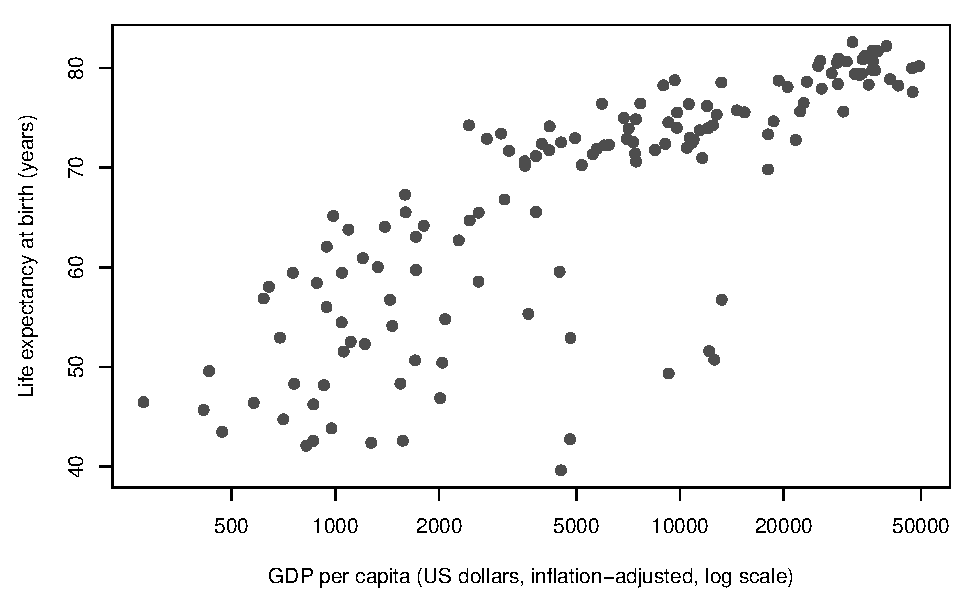
\includegraphics[width=\textwidth]{../output/figure1.pdf}
\caption{Life expectancy and GDP per capita, 2007}
\label{fig:scatter}

\medskip
\begin{minipage}{0.8\textwidth}\footnotesize
Notes: Each dot is a country. The horizontal axis is on a log scale.
Source: Gapminder, 2002.
\end{minipage}
\end{figure}

\section*{References}

\noindent Bryan, J. (2025). gapminder: Data from Gapminder. R package.
\url{https://doi.org/10.32614/CRAN.package.gapminder}

\medskip
\noindent Preston, S. H. (1975). The changing relation between mortality
and level of economic development. \emph{Population Studies} 29(2),
231--248. \url{https://doi.org/10.1080/00324728.1975.10410201}

\end{document}
